\section{FABRIK}

Forwards and Backwards Reaching Inverse Kinematics (FABRIK) is an algorithm that efficiently solves inverse kinematics for a number of joints in a system. Being a heuristic model, FABRIK avoids solving rotational matrices as conventional IK solvers, and instead translate the joints to a point on a line. This results in low computational requirements and and therefore faster computational speeds. A table comparing FABRIK to other IK solvers is shown in Figure \autoref{fig:table}. 

\begin{table}[H]
\centering
\label{fig:table}
\begin{tabular}{l|llll}
       & \textbf{Number of iterations} & \textbf{Matlab exe. time (sec)} & \textbf{Time per iteration (msec)} & \textbf{Iteration per second} \\ \hline
FABRIK & 15.461                        & 0.01328                         & 0.86                               & 1164                          \\
CCD    & 26.308                        & 0.12356                         & 4.69                               & 213                           \\
FTL    & 21.125                        & 0.002045                        & 0.97                               & 1033                          \\ \hline
\end{tabular}
\caption{Average results from different IK methods for a system with 10 joints}
\end{table}


The following section describes how FABRIK have been implemented and applied to the virtual da Vinci robot. It also describes the current problems with the algorithm and its implementation in Unreal Engine. 
The algorithm have been implemented according to Andreas Aristidou and Joan Lasenby \citep{FABRIK: A fast, iterative solver for the Inverse Kinematics problem}.  %Its in zotero. 

FABRIK is implemented in Unreal Engine's Animation Blueprint, but as this only allows to define preset animation sequences, it cannot be used to interact with in real-time. Standard Blueprint does not allow for bone or joint transformations and therefore a Poseable Mesh has to be created from the skeletal mesh of the robot in order to program bone behaviour. 

\subsection{FABRIK Algorithm Example}

Figure \ref{fig:ab} shows an example of a system consisting of four bones and an end effector. The goal of the algorithm is to get the outermost bone (P4) as close to the end effector (t) as possible and maintaining the original distance between each bone. 
The FABRIK algorithm starts by adding all bone lengths together to determine if the target is reachable or not. 
As FABRIK is a heuristic bone translation algorithm it starts at the end effector P4 and sets its position to the target's position as seen in Figure \ref{fig:ab}. The new heuristic joint is called P'4 

\begin{figure}[hbtp]
\centering
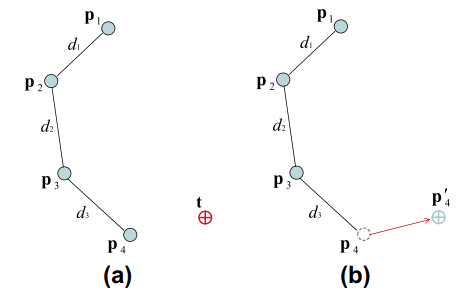
\includegraphics[width=1\textwidth]{FABRIK/ab}
\caption{First to stages in FABRIK; calculating positions based on end effector position and bone lengths}
\label{fig:ab}
\end{figure}

A line is then drawn from P'4 to P3, and since the original distance have to be maintained, P'3 is translated to somewhere on that line as seen in Figure \ref{}(c). The position on the line is calculated by 

$P'3 = (\hat{P3} - \hat{P4}) * d_{3}$

This procedure is then repeated for each bone in the system, creating a heuristic position for all joints, as seen in Figure \ref{fig:cd}. This results in the root bone(P1) being translated as well. 

\begin{figure}[hbtp]
\centering
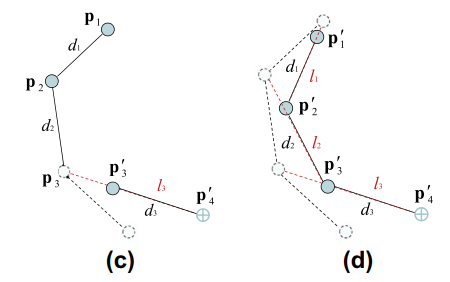
\includegraphics[width=1\textwidth]{FABRIK/cd}
\caption{Position of all joints are being recalculated, resulting in a slight offset from the root bone's original position}
\label{fig:cd}
\end{figure}

The root joint is then moved back to its initial position and the same process now repeats in the other direction (root to outer joint) as seen in Figure \ref{fig:ef}.

\begin{figure}[hbtp]
 \centering
 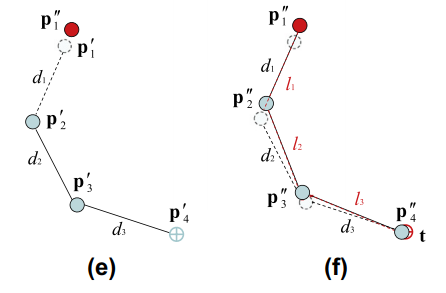
\includegraphics[width=1\textwidth]{FABRIK/ef}
 \caption{The same process now repeats, now where the root bone is moved back to its original position. These processes repeat until the end effector is within a set distance to the target}
 \label{fig:ef}
 \end{figure}
  
This process is then repeated until the end effector hits the target or gets sufficiently close. 

\subsection{Implementation in Unreal Engine}

For implementation purposes, Unreal's Poseable Mesh blueprint was used to translate the bones toward the target. Below is a table of the variables used by the blueprint with a description of its use. 

% Please add the following required packages to your document preamble:
% \usepackage[table,xcdraw]{xcolor}
% If you use beamer only pass "xcolor=table" option, i.e. \documentclass[xcolor=table]{beamer}
\begin{table}[]
\centering
\caption{Table of the important variables of FABRIK}
\begin{tabular}{l|lll}
\rowcolor[HTML]{BBDAFF} 
{\color[HTML]{000000} \textbf{Name of Variable}} & {\color[HTML]{000000} \textbf{Type}} & {\color[HTML]{000000} \textbf{Use}}                                                                                                                                                                                            & {\color[HTML]{000000} \textbf{Static}} \\ \hline
\textbf{Arm1}                                    & Array of Bones                       & Contains all the bones of the robot arm. Used to reference.                                                                                                                                                                    & Yes                                    \\
\textbf{BoneLocations}                           & Array of Positions                   & \begin{tabular}[c]{@{}l@{}}Contains all the bones positions in world space. \\ Used in the start to calculate the original distances \\ between joints and updated later when new positions \\ are calculated.\end{tabular}    & No                                     \\
\textbf{Lengths}                                 & Array of Bone Lengths                & \begin{tabular}[c]{@{}l@{}}The array of bone lengths are constant and is needed to \\ calculate heuristics.\end{tabular}                                                                                                       & Yes                                    \\
\textbf{Target}                                  & Object                               & \begin{tabular}[c]{@{}l@{}}The actual object that the end effector will try to reach. \\ This is a red semi transparent cube. Used to set the end\\ effector's position to the target and to calculate proximity.\end{tabular} & Yes                                    \\
\textbf{Origin1}                                 & Position                             & \begin{tabular}[c]{@{}l@{}}The root's original position. Used in the start of the "Forwards"\\ part where the root's position is set to its original position.\end{tabular}                                                    & Yes                                    \\
                                                 &                                      &                                                                                                                                                                                                                                &                                        \\
                                                 &                                      &                                                                                                                                                                                                                                &                                        \\
                                                 &                                      &                                                                                                                                                                                                                                &                                        \\
                                                 &                                      &                                                                                                                                                                                                                                &                                       
\end{tabular}
\label{tab:table}
\end{table}

The code is split up in four main parts;

\begin{itemize}
\item BeginPlay
\item OutOfReach
\item Backwards (Heuristics)
\item Forwards (Positioning joints)
\end{itemize}

BeginPlay initializes and calculates all of the variables in \autoref{tab:table}. OutOfReach determines if the target is out of reach and, if so, stretches all bones in the target's direction. 
Backwards handles the heuristics of the algorithm and the flow of this program can be seen in Figure \ref{fig:flow}. The Forwards then calculates the real position of the joint and sets the position of the joint in world space. The forwards look like the flow in Figure \ref{fig:flow} the only difference being a positive for loop and the order in the "pos" calculation.

\begin{figure}[H]
\centering
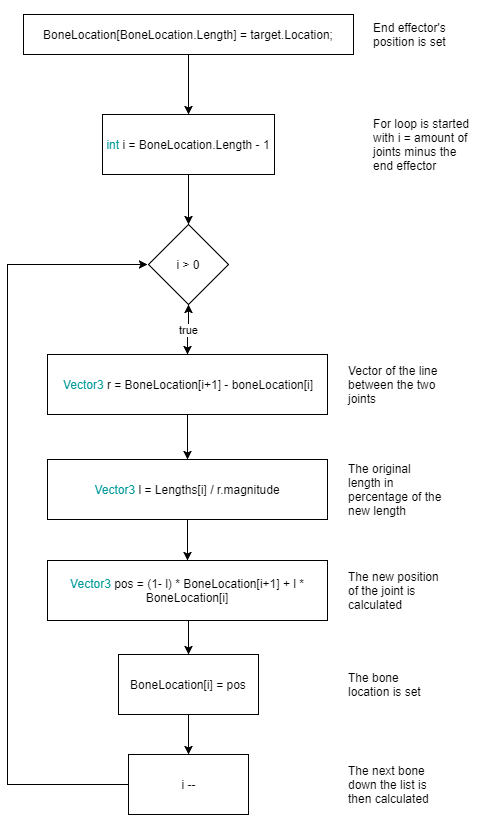
\includegraphics[width=1\textwidth]{FABRIK/Flowchart.png}
\caption{Caption here}
\label{fig:flow}
\end{figure}

\subsection{Results}

The results of this implementation is seen in \autoref{fig:results}. It is clear that the implementation did not work as intended, as a small movement of the target transforms the bones with this magnitude. This is the case no matter what direction the target is moved. 


\begin{figure}[hbtp]
\begin{subfigure}[b]{0.48\textwidth}
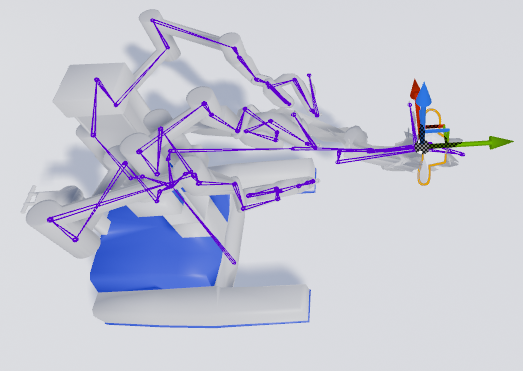
\includegraphics[width=1\textwidth]{FABRIK/Robot_state1.PNG}
\caption{The robot and its bones in one state with the target visible}
\end{subfigure} 
\begin{subfigure}[b]{0.48\textwidth}
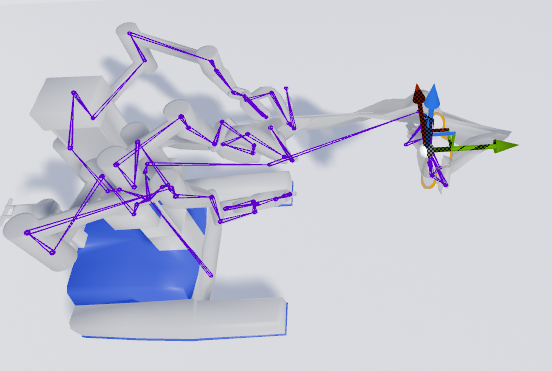
\includegraphics[width=1\textwidth]{FABRIK/Robot_state2.PNG}
\caption{The robot in another state where the target has moved slightly}
\end{subfigure}
\label{fig:results}
\end{figure}


Looking at the target out of reach as seen in \autoref{fig:outofreach}, the IK acts as expected and only points towards the target without any radical movements. 

\begin{figure}[hbtp]
\centering
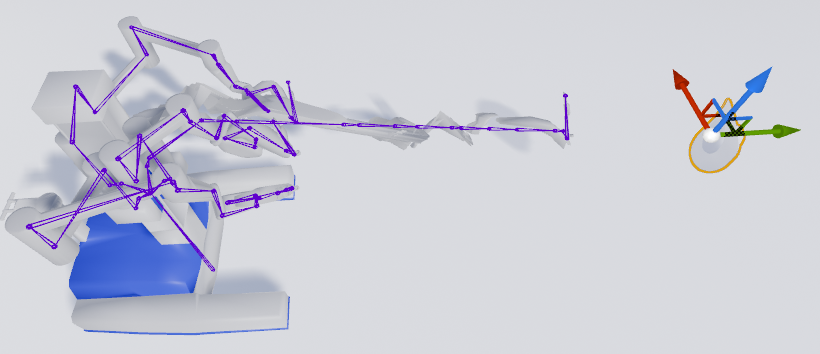
\includegraphics[width=1\textwidth]{FABRIK/Robot_OutOfReach.PNG}
\caption{The arms when the target is out of reach}
\end{figure}

One of the reasons the FABRIK acts radically when the target is in reach might be because of the Blueprint implementation. Blueprints lack several basic features such as reverse for loops. This leads to more complexity of the code, since these have to be programmed in blueprints. As complexity increases debugging also gets more difficult. 
Due to time constraints the cyclic coordinate descent algorithm was implemented instead. 